\documentclass[12pt,a4paper]{article}

\usepackage{ctex}
\usepackage{amsmath,amssymb}
\usepackage{graphicx}
\usepackage{xcolor}
\usepackage{eso-pic}
\usepackage{geometry}
\usepackage{enumitem}
\usepackage{fancyhdr}
\usepackage{multicol}

\geometry{left=2cm,right=2cm,top=2.5cm,bottom=2.5cm}

\title{\textbf{贺昱超练习卷}}
\author{}
\date{\today}

% --- 用户自定义水印代码开始 ---
\newcommand{\WMText}{贺昱超学习资料}
\newcommand{\WMScale}{2.28}
\newcommand{\WMAngle}{45}
\colorlet{WMColor}{black!8}

\AddToShipoutPictureBG{%
  \AtPageLowerLeft{%
    \put(\LenToUnit{0.66\paperwidth},\LenToUnit{0.70\paperheight}){%
      \rotatebox{\WMAngle}{\scalebox{\WMScale}{\textcolor{WMColor}{\WMText}}}%
    }%
    \put(\LenToUnit{0.33\paperwidth},\LenToUnit{0.50\paperheight}){%
      \rotatebox{\WMAngle}{\scalebox{\WMScale}{\textcolor{WMColor}{\WMText}}}%
    }%
    \put(\LenToUnit{0.66\paperwidth},\LenToUnit{0.30\paperheight}){%
      \rotatebox{\WMAngle}{\scalebox{\WMScale}{\textcolor{WMColor}{\WMText}}}%
    }%
  }%
}
% --- 用户自定义水印代码结束 ---

\pagestyle{fancy}
\fancyhf{}
\lhead{贺昱超练习卷}
\rhead{Physics Practice}
\cfoot{\thepage}

\setlength{\parindent}{0pt}
\setlength{\parskip}{0.6em}

% --- Vocabulary box ---
\newcommand{\vocab}[1]{
\begin{quote}
\small
\textbf{Vocabulary:} #1
\end{quote}
}

\begin{document}

\maketitle

\begin{center}
\Large MCQ 4 points for each question
\end{center}

\section*{Multiple Choice Questions}

\subsection*{1}

An object is initially at the origin. The object changes its position to the right by 4 units. The object then changes its position to the left by 3 units. Which of the following correctly indicates the magnitude of the object's change in position and provides a valid justification?

\vocab{
origin：原点；
position：位置；
to the right：向右；
to the left：向左；
magnitude：大小；
change in position：位置变化 / 位移；
valid justification：有效理由；
opposite directions：相反方向；
opposite signs：相反符号。
}

\begin{enumerate}[label=(\Alph*)]
    \item 1 unit, because in one dimension vectors with opposite directions have opposite signs.
    \item 1 unit, because the magnitude of the difference of two vectors is always equal to the difference between the magnitudes of the vectors.
    \item 7 units, because the magnitude of the sum of two vectors is always equal to the sum of the magnitudes of the vectors.
    \item 7 units, because the object moves a distance of 4 units followed by a distance of 3 units.
\end{enumerate}

\subsection*{2}

\begin{center}
\begin{tabular}{|c|c|c|}
\hline
Car & Velocity & Acceleration \\
\hline
A & $+6.0\ \text{m/s}$ & $+1.5\ \text{m/s}^2$ \\
\hline
B & $-7.0\ \text{m/s}$ & $+2.0\ \text{m/s}^2$ \\
\hline
C & $+8.0\ \text{m/s}$ & $-2.5\ \text{m/s}^2$ \\
\hline
D & $-9.0\ \text{m/s}$ & $-1.0\ \text{m/s}^2$ \\
\hline
\end{tabular}
\end{center}

Cars A, B, C, and D are moving along a straight track. The table indicates their velocities and accelerations at the same instant. Which car has the acceleration with the greatest magnitude?

\vocab{
straight track：直线轨道；
velocity：速度；
acceleration：加速度；
at the same instant：在同一时刻；
magnitude：大小；
greatest magnitude：最大大小；
positive / negative：正的 / 负的。
}

\begin{enumerate}[label=(\Alph*)]
    \item Car A
    \item Car B
    \item Car C
    \item Car D
\end{enumerate}

\subsection*{3}

Vectors $\vec{A}$ and $\vec{B}$ are parallel to the $x$-axis. Vector $\vec{C}$ is defined to be the vector sum of $\vec{A}$ and $\vec{B}$, or
\[
\vec{C}=\vec{A}+\vec{B}.
\]
Vector $\vec{C}$ has the same direction as vector $\vec{B}$, and the magnitudes of $\vec{B}$ and $\vec{C}$ are related by
\[
|\vec{B}|>|\vec{C}|.
\]
Which of the following claims is correct about the relative directions and magnitudes of vectors $\vec{A}$ and $\vec{B}$?

\vocab{
vector：向量；
parallel to：平行于；
$x$-axis：$x$轴；
vector sum：向量和；
same direction：相同方向；
opposite directions：相反方向；
magnitude：大小；
relative directions：相对方向。
}

\begin{enumerate}[label=(\Alph*)]
    \item $|\vec{A}|>|\vec{B}|$ and the vectors have the same direction.
    \item $|\vec{A}|>|\vec{B}|$ and the vectors have opposite directions.
    \item $|\vec{A}|<|\vec{B}|$ and the vectors have the same direction.
    \item $|\vec{A}|<|\vec{B}|$ and the vectors have opposite directions.
\end{enumerate}

\subsection*{4}

A car is driving east on a straight, level road with a speed of $20\ \text{m/s}$ when it begins to accelerate eastward at a constant rate. After $5\ \text{s}$ the car has a speed of $40\ \text{m/s}$ to the east. The acceleration of the car during the $5\ \text{s}$ time interval is

\vocab{
east：向东；
straight, level road：笔直平坦的道路；
speed：速率；
accelerate：加速；
eastward：向东地；
constant rate：恒定速率 / 恒定变化率；
time interval：时间间隔；
acceleration：加速度。
}

\begin{enumerate}[label=(\Alph*)]
    \item $4\ \text{m/s}^2$
    \item $8\ \text{m/s}^2$
    \item $20\ \text{m/s}^2$
    \item $30\ \text{m/s}^2$
\end{enumerate}

\subsection*{5}

An object on a straight, horizontal track with an initial positive velocity undergoes a constant acceleration of $-5\ \text{m/s}^2$ for $4$ seconds. Which of the following is the change in velocity of the object during this interval?

\vocab{
straight, horizontal track：水平直线轨道；
initial positive velocity：初始正速度；
undergo：经历；
constant acceleration：恒定加速度；
change in velocity：速度变化量；
during this interval：在这段时间内。
}

\begin{enumerate}[label=(\Alph*)]
    \item $-20\ \text{m/s}$
    \item $-5\ \text{m/s}$
    \item $-1.2\ \text{m/s}$
    \item $0\ \text{m/s}$
\end{enumerate}

\subsection*{6}

\begin{center}

\includegraphics[width=0.45\textwidth]{6.png}
\end{center}

The graph above represents position $x$ versus time $t$ for an object being acted on by a constant force. The average speed during the interval between $1\ \text{s}$ and $2\ \text{s}$ is most nearly

\vocab{
position：位置；
time：时间；
position versus time graph：位置-时间图像；
acted on by：受到……作用；
constant force：恒力；
average speed：平均速率；
interval：区间；
most nearly：最接近。
}

\begin{enumerate}[label=(\Alph*)]
    \item $2\ \text{m/s}$
    \item $4\ \text{m/s}$
    \item $5\ \text{m/s}$
    \item $6\ \text{m/s}$
    \item $8\ \text{m/s}$
\end{enumerate}

\subsection*{7}

\begin{center}

\includegraphics[width=0.75\textwidth]{7.png}
\end{center}

Car A is traveling to the right at a constant velocity $v_A$. At time $t=0$, it passes Car B, which is at rest. At the same time $(t=0)$, Car B begins to accelerate with a constant acceleration of magnitude $a_B$, as shown in Figure 1. Car B has a velocity of $v_B$ when it reaches the same position as Car A at time $t=t_f$, as shown in Figure 2. Which of the following, if any, is an expression for the time it takes for Car B to catch up to Car A?

\vocab{
travel to the right：向右运动；
constant velocity：恒定速度；
at rest：静止；
accelerate：加速；
constant acceleration：恒定加速度；
magnitude：大小；
same position：相同位置；
catch up to：追上；
expression：表达式。
}

\begin{enumerate}[label=(\Alph*)]
    \item $\dfrac{v_A}{a_B}$
    \item $\dfrac{2v_A}{a_B}$
    \item $\dfrac{2v_A^2}{a_B}$
    \item It cannot be determined without knowing the distance traveled by the cars.
\end{enumerate}

\subsection*{8}

\begin{center}

\includegraphics[width=0.45\textwidth]{8.png}
\end{center}

A cart moves along a horizontal, one-dimensional track according to the position-time graph shown, where positive positions represent locations to the right of the origin. Which of the following statements correctly describe the cart's instantaneous velocity at time $5\ \text{s}$?

\vocab{
cart：小车；
horizontal：水平的；
one-dimensional track：一维轨道；
position-time graph：位置-时间图像；
positive positions：正位置；
to the right of the origin：在原点右侧；
instantaneous velocity：瞬时速度；
moving left / right：向左 / 向右运动；
speed：速率。
}

\begin{enumerate}[label=(\Alph*)]
    \item The cart is moving left with speed $1.0\ \text{cm/s}$.
    \item The cart is moving right with speed $1.0\ \text{cm/s}$.
    \item The cart is moving left with speed $0.5\ \text{cm/s}$.
    \item The cart is moving right with speed $0.5\ \text{cm/s}$.
\end{enumerate}

\subsection*{9}

\begin{center}

\includegraphics[width=0.75\textwidth]{9.png}
\end{center}

The graphs represent the speed of a ball thrown downward as a function of time near the surface of two planets. Which of the following correctly relates the acceleration $a_1$ of the ball near the surface of Planet 1 and the acceleration $a_2$ of the ball near the surface of Planet 2?

\vocab{
speed：速率；
thrown downward：向下抛出；
as a function of time：作为时间的函数；
near the surface：在表面附近；
planet：行星；
acceleration：加速度；
correctly relates：正确比较；
greater than：大于。
}

\begin{enumerate}[label=(\Alph*)]
    \item $a_1>a_2>0$
    \item $a_2>a_1>0$
    \item $(a_1=a_2)>0$
    \item $a_1=a_2=0$
\end{enumerate}

\subsection*{10}

\begin{center}

\includegraphics[width=0.55\textwidth]{10.png}
\end{center}

On another planet, a ball is in free fall after being released from rest at time $t=0$. A graph of the height of the ball above the planet's surface as a function of time $t$ is shown. The acceleration due to gravity on the planet is most nearly

\vocab{
free fall：自由落体；
released from rest：从静止释放；
height：高度；
above the surface：在表面上方；
as a function of time：作为时间的函数；
acceleration due to gravity：重力加速度；
most nearly：最接近。
}

\begin{enumerate}[label=(\Alph*)]
    \item $8\ \text{m/s}^2$
    \item $16\ \text{m/s}^2$
    \item $20\ \text{m/s}^2$
    \item $40\ \text{m/s}^2$
\end{enumerate}

\subsection*{11}

An automobile traveling on a straight, level road has an initial speed $v$ when the brakes are applied. In coming to rest with a constant acceleration, it travels a distance $x$. How far would the automobile travel in coming to rest if it had the same acceleration but an initial speed $2v$?

\vocab{
automobile：汽车；
straight, level road：笔直平坦的道路；
initial speed：初速度；
brakes are applied：刹车被使用；
come to rest：停下来；
constant acceleration：恒定加速度；
travel a distance：行驶一段距离；
same acceleration：相同加速度。
}

\begin{enumerate}[label=(\Alph*)]
    \item $\dfrac{1}{4}x$
    \item $\dfrac{1}{2}x$
    \item $x$
    \item $2x$
    \item $4x$
\end{enumerate}

\subsection*{12}

An object is thrown with a horizontal velocity of $20\ \text{m/s}$ from a cliff that is $125\ \text{m}$ above level ground. If air resistance is negligible, the time that it takes the object to fall to the ground from the cliff is most nearly

\vocab{
horizontal velocity：水平速度；
cliff：悬崖；
above level ground：高于水平地面；
air resistance：空气阻力；
negligible：可忽略的；
fall to the ground：落到地面；
most nearly：最接近。
}

\begin{enumerate}[label=(\Alph*)]
    \item $3\ \text{s}$
    \item $5\ \text{s}$
    \item $6\ \text{s}$
    \item $12\ \text{s}$
    \item $25\ \text{s}$
\end{enumerate}

\subsection*{13}

\begin{center}

\includegraphics[width=0.55\textwidth]{13.png}
\end{center}

An object is sliding to the right along a straight line on a horizontal surface. The graph shows the object's velocity as a function of time. What is the object's displacement during the time depicted in the graph?

\vocab{
slide：滑动；
to the right：向右；
straight line：直线；
horizontal surface：水平表面；
velocity as a function of time：速度关于时间的函数；
displacement：位移；
during the time depicted：在图中所示时间内。
}

\begin{enumerate}[label=(\Alph*)]
    \item $0\ \text{m}$
    \item $1\ \text{m}$
    \item $8\ \text{m}$
    \item $16\ \text{m}$
\end{enumerate}

\subsection*{14}

\begin{center}

\includegraphics[width=0.45\textwidth]{14.png}
\end{center}

The diagram shows the directions and magnitudes of the forces exerted on a puck on a horizontal surface. What is the magnitude of the vector sum of the forces exerted on the puck?

\vocab{
diagram：图示；
directions：方向；
magnitudes：大小；
force：力；
exerted on：施加在……上；
puck：冰球 / 圆盘；
horizontal surface：水平表面；
vector sum：向量和；
magnitude of the vector sum：合力大小。
}

\begin{enumerate}[label=(\Alph*)]
    \item $3\ \text{N}$
    \item $4\ \text{N}$
    \item $5\ \text{N}$
    \item $7\ \text{N}$
\end{enumerate}

\subsection*{15}

A projectile is launched from level ground with initial velocity $v_0$, at an angle $\theta$ above horizontal. Which of the following is an expression for the total time the projectile is in the air?

\vocab{
projectile：抛体；
launched：发射；
level ground：水平地面；
initial velocity：初速度；
angle above horizontal：与水平方向成角；
expression：表达式；
total time：总时间；
in the air：在空中。
}

\begin{enumerate}[label=(\Alph*)]
    \item $t=\dfrac{v_0\cos\theta}{g}$
    \item $t=\dfrac{2v_0\cos\theta}{g}$
    \item $t=\dfrac{v_0\sin\theta}{g}$
    \item $t=\dfrac{2v_0\sin\theta}{g}$
\end{enumerate}

\newpage

\section*{Free Response Questions}

\subsection*{16 \quad [12 points]}

A particle is moving in one dimension along the $x$-axis. The position of the particle is given, for any time, by the following position function:
\[
x(t)=3t^2+2.
\]

\vocab{
particle：粒子；
one dimension：一维；
along the $x$-axis：沿$x$轴；
position function：位置函数；
evaluate：计算；
average velocity：平均速度；
starting at：从……开始；
$\Delta t$：时间间隔；
interpret：解释；
physical meaning：物理意义。
}

\begin{enumerate}[label=(\alph*)]
    \item Evaluate the average velocity of the particle starting at $t=2\ \text{s}$ for
    \[
    \Delta t=1,\ 0.5,\ 0.2,\ 0.1,\ 0.01,\ 0.001\ \text{s}.
    \]
    \item Interpret the physical meaning of your results for part (a).
\end{enumerate}

\subsection*{17 \quad [12 points]}

A football quarterback throws a pass to a receiver at an angle of $25^\circ$ to the horizontal and at an initial velocity of $25\ \text{m/s}$. The receiver is initially at rest $30\ \text{m}$ from the quarterback. The instant the ball is thrown, the receiver runs at a constant velocity to catch the pass. In what direction and at what speed should he run?

\vocab{
football quarterback：四分卫；
receiver：接球员；
pass：传球；
angle to the horizontal：与水平方向的夹角；
initial velocity：初速度；
initially at rest：最初静止；
the instant：在……瞬间；
constant velocity：恒定速度；
catch the pass：接住传球；
direction：方向；
speed：速率。
}

\subsection*{18 \quad [16 points]}

A $0.50\ \text{kg}$ cart moves on a straight horizontal track. The graph of velocity $v_x$ versus time $t$ for the cart is given below.

\vocab{
cart：小车；
straight horizontal track：水平直线轨道；
velocity versus time graph：速度-时间图像；
at rest：静止；
speed：速率；
magnitude of velocity：速度大小；
increasing：增加；
horizontal position：水平位置；
sketch：画草图；
acceleration versus time graph：加速度-时间图像；
constant horizontal velocity：恒定水平速度；
end of the track：轨道末端；
hits the floor：撞到地面；
neglecting air resistance：忽略空气阻力；
horizontal distance：水平距离；
kinetic energy：动能；
immediately before：就在……之前。
}

\begin{center}
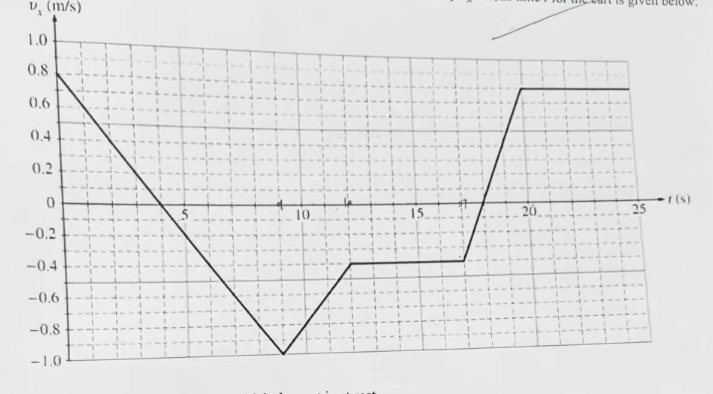
\includegraphics[width=0.85\textwidth]{18.png}
\end{center}

\begin{enumerate}[label=(\alph*)]
    \item Indicate every time $t$ for which the cart is at rest.

    \item Indicate every time interval for which the speed, magnitude of velocity, of the cart is increasing.

    \item Determine the horizontal position $x$ of the cart at $t=9.0\ \text{s}$ if the cart is located at $x=2.0\ \text{m}$ at $t=0$.

    \item On the axes below, sketch the acceleration $a$ versus time $t$ graph for the motion of the cart from $t=0$ to $t=25\ \text{s}$.

    \begin{center}
    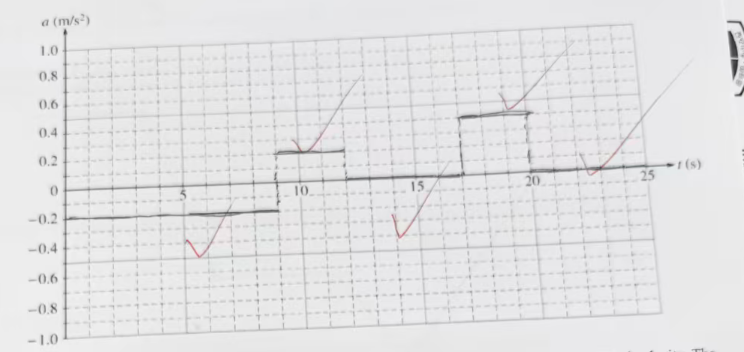
\includegraphics[width=0.85\textwidth]{18d.png}
    \end{center}

    \item From $t=25\ \text{s}$ until the cart reaches the end of the track, the cart continues with constant horizontal velocity. The cart leaves the end of the track and hits the floor, which is $0.40\ \text{m}$ below the track. Neglecting air resistance, determine each of the following.

    \begin{enumerate}[label=\roman*.]
        \item The time from when the cart leaves the track until it first hits the floor.
        \item The horizontal distance from the end of the track to the point at which the cart first hits the floor.
        \item The kinetic energy of the cart immediately before it hits the floor.
    \end{enumerate}
\end{enumerate}

\end{document}